\documentclass[]{book}
\usepackage{lmodern}
\usepackage{amssymb,amsmath}
\usepackage{ifxetex,ifluatex}
\usepackage{fixltx2e} % provides \textsubscript
\ifnum 0\ifxetex 1\fi\ifluatex 1\fi=0 % if pdftex
  \usepackage[T1]{fontenc}
  \usepackage[utf8]{inputenc}
\else % if luatex or xelatex
  \ifxetex
    \usepackage{mathspec}
  \else
    \usepackage{fontspec}
  \fi
  \defaultfontfeatures{Ligatures=TeX,Scale=MatchLowercase}
\fi
% use upquote if available, for straight quotes in verbatim environments
\IfFileExists{upquote.sty}{\usepackage{upquote}}{}
% use microtype if available
\IfFileExists{microtype.sty}{%
\usepackage{microtype}
\UseMicrotypeSet[protrusion]{basicmath} % disable protrusion for tt fonts
}{}
\usepackage[margin=1in]{geometry}
\usepackage{hyperref}
\hypersetup{unicode=true,
            pdftitle={Conferences 2016},
            pdfauthor={Sungpil Han},
            pdfborder={0 0 0},
            breaklinks=true}
\urlstyle{same}  % don't use monospace font for urls
\usepackage{natbib}
\bibliographystyle{plainnat}
\usepackage{longtable,booktabs}
\usepackage{graphicx,grffile}
\makeatletter
\def\maxwidth{\ifdim\Gin@nat@width>\linewidth\linewidth\else\Gin@nat@width\fi}
\def\maxheight{\ifdim\Gin@nat@height>\textheight\textheight\else\Gin@nat@height\fi}
\makeatother
% Scale images if necessary, so that they will not overflow the page
% margins by default, and it is still possible to overwrite the defaults
% using explicit options in \includegraphics[width, height, ...]{}
\setkeys{Gin}{width=\maxwidth,height=\maxheight,keepaspectratio}
\IfFileExists{parskip.sty}{%
\usepackage{parskip}
}{% else
\setlength{\parindent}{0pt}
\setlength{\parskip}{6pt plus 2pt minus 1pt}
}
\setlength{\emergencystretch}{3em}  % prevent overfull lines
\providecommand{\tightlist}{%
  \setlength{\itemsep}{0pt}\setlength{\parskip}{0pt}}
\setcounter{secnumdepth}{5}
% Redefines (sub)paragraphs to behave more like sections
\ifx\paragraph\undefined\else
\let\oldparagraph\paragraph
\renewcommand{\paragraph}[1]{\oldparagraph{#1}\mbox{}}
\fi
\ifx\subparagraph\undefined\else
\let\oldsubparagraph\subparagraph
\renewcommand{\subparagraph}[1]{\oldsubparagraph{#1}\mbox{}}
\fi
\usepackage{booktabs}
\usepackage{longtable}
\usepackage{framed,color}
\usepackage{kotex}

\definecolor{shadecolor}{RGB}{248,248,248}

\ifxetex
  \usepackage{letltxmacro}
  \setlength{\XeTeXLinkMargin}{1pt}
  \LetLtxMacro\SavedIncludeGraphics\includegraphics
  \def\includegraphics#1#{% #1 catches optional stuff (star/opt. arg.)
    \IncludeGraphicsAux{#1}%
  }%
  \newcommand*{\IncludeGraphicsAux}[2]{%
    \XeTeXLinkBox{%
      \SavedIncludeGraphics#1{#2}%
    }%
  }%
\fi

\newenvironment{rmdblock}[1]
  {\begin{shaded*}
  \begin{itemize}
  \renewcommand{\labelitemi}{
    \raisebox{-.7\height}[0pt][0pt]{
      {\setkeys{Gin}{width=3em,keepaspectratio}\includegraphics{images/#1}}
    }
  }
  \item
  }
  {
  \end{itemize}
  \end{shaded*}
  }
\newenvironment{rmdnote}
  {\begin{rmdblock}{note}}
  {\end{rmdblock}}
\newenvironment{rmdcaution}
  {\begin{rmdblock}{caution}}
  {\end{rmdblock}}
\newenvironment{rmdimportant}
  {\begin{rmdblock}{important}}
  {\end{rmdblock}}
\newenvironment{rmdtip}
  {\begin{rmdblock}{tip}}
  {\end{rmdblock}}
\newenvironment{rmdwarning}
  {\begin{rmdblock}{warning}}
  {\end{rmdblock}}

%%% Use protect on footnotes to avoid problems with footnotes in titles
\let\rmarkdownfootnote\footnote%
\def\footnote{\protect\rmarkdownfootnote}

%%% Change title format to be more compact
\usepackage{titling}

% Create subtitle command for use in maketitle
\newcommand{\subtitle}[1]{
  \posttitle{
    \begin{center}\large#1\end{center}
    }
}

\setlength{\droptitle}{-2em}
  \title{Conferences 2016}
  \pretitle{\vspace{\droptitle}\centering\huge}
  \posttitle{\par}
  \author{Sungpil Han}
  \preauthor{\centering\large\emph}
  \postauthor{\par}
  \predate{\centering\large\emph}
  \postdate{\par}
  \date{2016-07-13}

\begin{document}
\maketitle

{
\setcounter{tocdepth}{1}
\tableofcontents
}
\chapter{Introduction}\label{introduction}

\chapter{2016 KSCPT}\label{kscpt}

\begin{figure}[htbp]
\centering
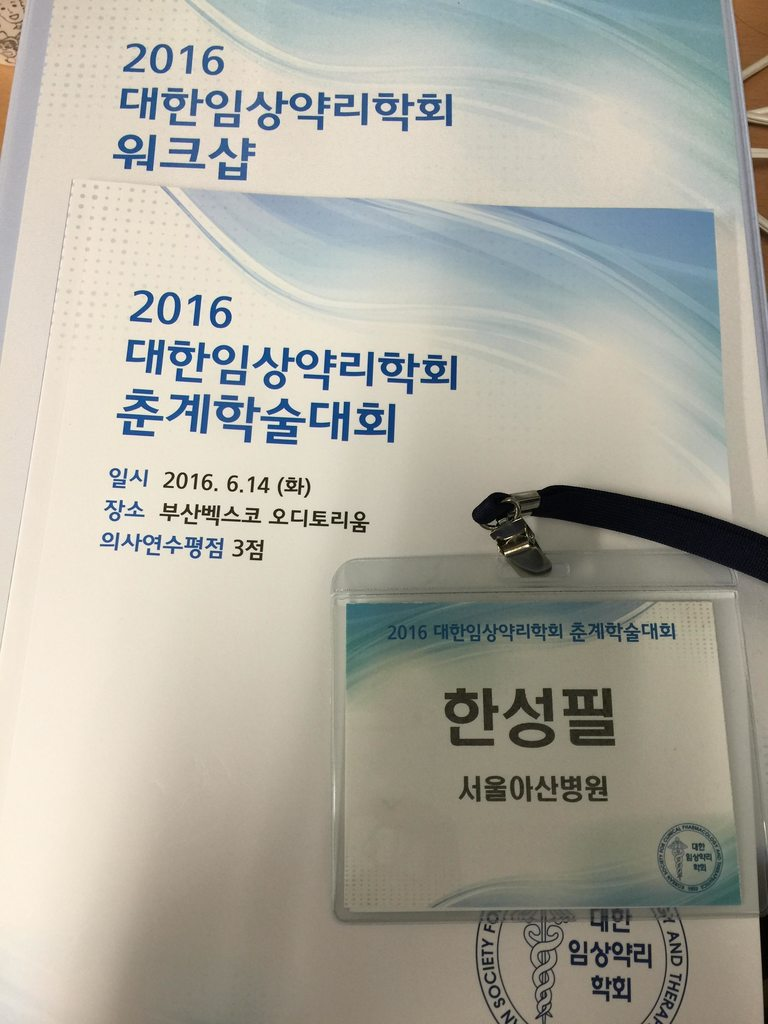
\includegraphics{images/2016KSCPT.jpg}
\caption{Materials}
\end{figure}

\section{Opening Remark}\label{opening-remark}

\begin{itemize}
\tightlist
\item
  Yil-Seob Lee (president of KSCPT)
\end{itemize}

\section{First Session}\label{first-session}

\begin{itemize}
\tightlist
\item
  Chair : Deborah Chee(KoNECT)
\end{itemize}

\subsection{13:20\textasciitilde{}14:00 Precision Medicine: A Clinical
Pharmacological
Perspective}\label{precision-medicine-a-clinical-pharmacological-perspective}

\begin{itemize}
\tightlist
\item
  Speaker: \href{https://en.wikipedia.org/wiki/Munir_Pirmohamed}{Munir
  Pirmohamed} (University of Liverpool, UK)
\item
  Fava beans - Favism G6PD deficiency - withrawal of antimalarials
\item
  2015 Obama Precision Medicine \$215m / 2016 China \$8b
\item
  Phenotypic definition(current standard) - Molecular definition
  (disease stratification) - Drug variability
\item
  Mandatory genomic testing - EMA SmPC
\item
  Pharmacogenomics Journal (2015) 1-10
\item
  Crizotinib vs CTx in advanced ALK+ lung cancer (NEJM 2013)
\item
  Novel trial design (Nature 2015)
\end{itemize}

\begin{enumerate}
\def\labelenumi{\arabic{enumi}.}
\tightlist
\item
  Umbrella trial (single tumor - multiple arm - multiple drugs)
\item
  Basket study
\end{enumerate}

\begin{itemize}
\tightlist
\item
  Support of humen genetic evidence for approved drug indication (Nature
  Genetics)
\item
  Sclerosteosis - skeletal overgrowth and syndactyly, AR , mutations in
  SOST gene - target sclerostin
\item
  anti-sclerostin Ab (ROMOSOZUMAB, BLOSOZUMAB) - bone density increase -
  mouse
\item
  New cardiovascular targets
\item
  PCSK9 - GOF-\textgreater{}LDL-C increase \& CVD
\item
  ANGPTL4
\item
  HLA-genotype and carbamazepine-induced cutaneous ADR: systemic review
  (CPT,2012)
\item
  ITCH (Drug hypersensitivity)
\item
  Phase I, II - very strong association (Manhattan plot) - GWAS -
  ALK(germline polymorphism-\textgreater{} T cell expansion)
\item
  SJS GWAS (Genin 2011)
  \url{http://www.ncbi.nlm.nih.gov/pubmed/21801394}
\item
  Skin, Liver
\item
  CBZ-induced hypersensitivity vs CBZ-tolerant patients
\item
  HLA-A*31:01(thirtyone o one)
\item
  HLA and ADR
\item
  The effect of pharmacogenetic profiling with a clinical decision
  support tool on healthcare resource utilization and estimated costs in
  the elderly exposed to polypharmacy. (2016)
  \url{http://www.ncbi.nlm.nih.gov/pubmed/26478982}
\item
  Somatic genomes -\textgreater{} microbiome is also important
\item
  Digoxin and antibiotics (1981, NEJM) -\textgreater{} (2013 Science)
  Cardiac drug inactivation by human gut bacteria
\item
  Microbiome and Cancer Immunotherapy - Snyder, Science Nov 2015
\item
  Two books introduced.
\end{itemize}

\begin{enumerate}
\def\labelenumi{\arabic{enumi}.}
\tightlist
\item
  Prescription for nhs
\item
  clinical pharma dynamic medical specialty
\end{enumerate}

\subsection{14:00\textasciitilde{}14:30 The role of pharmacogenomics in
drug development, regulatory review and clinical
practice}\label{the-role-of-pharmacogenomics-in-drug-development-regulatory-review-and-clinical-practice}

\begin{itemize}
\tightlist
\item
  Speaker: Shiew-Mei Huang (North Potomac, MD, USA)
\item
  CPIC (Clinical pharmacogenetics guidelines)
\item
  IFNL3(IL28B) HCV treatment Favorable response = 77\% Asian (Genotype
  CC)
\item
  Paving the way for Personalized Medicine (Oct 2013)
\item
  Avacavir HLA-B*5701 (RCT) Utility of pharmacogenetic tests
\item
  Munir mentioned - CBZ \& HLA-B*1502
\item
  ASCO meeting - CTx vs Targeted therapy - Umbrella study
\item
  Drug labeling ``FDA-approved test''
\item
  XALKORI - Crizotinib and ALK
\item
  CPT Feb 2016 - Precision Medicine , ``Companion Diagnostics''
  Something unique to conduct , ``Complementary diagnostics''
\item
  Eliglustat and CYP2D6 , Drug labeling
\item
  Center for Device
\item
  Integral to the future of personalized or precision medicine
\item
  NGS
\item
  PrecisionFDA initiative
\item
  23andMe - Drug response , Confidence
\item
  Cleared or approved FDA
\item
  CLIA-certified laboratory
\end{itemize}

\subsubsection{My Question}\label{my-question}

\begin{itemize}
\tightlist
\item
  One NGS - individual test to is there a review of all-in-one Test in
  progress?
\end{itemize}

\subsection{14:30\textasciitilde{}15:00 The Liver-Gut Microbiota Axis
Modulates Inter-Individual Variability in Xenobiotic Disposition and
Toxicology}\label{the-liver-gut-microbiota-axis-modulates-inter-individual-variability-in-xenobiotic-disposition-and-toxicology}

\begin{itemize}
\tightlist
\item
  Speaker: Eric Chun Yong Chan (National University of Singapore)
\item
  Liver - major organ for disposition and detoxification
\item
  60\% (explanble) vs 40\% (how about this?) - superorganism
\item
  400 different species (\textasciitilde{}1.5kg)
\item
  Haiser (2012, Science) Gut microbe - drug, host interaction
\item
  TOC: 1 DMD paper , 2 in-house project
\item
  DMD - reduction, hydrolysis
\item
  absorption - simvastatin - poor responder, average, good 10\% 80\%
  10\%

  \begin{itemize}
  \tightlist
  \item
    OATP1B1 in liver and intestine
  \item
    Possibility of competition between simvastatin and bile acids for
    hepatic uptake by transporter
  \item
    antibiotics - nitro-reduction by gut microbiota inhibition
  \item
    Therapeutic fficacy - DDI
  \end{itemize}
\item
  PCA analysis PNAS 2009 - significant differences in concentration
\item
  PNAS 2009 inverse corr - p-cresol \textless{}-\textgreater{} AAP
\item
  2nd part - Tacrine - first drug approved for AD. Toxicological
  manifestation - increased AST/ALT
\item
  Interindividual variability. why?
\item
  Tacrine metabolism - hydroxylation / glucuronide
\item
  mitochondrial toxicity and hypoxia-reoxygenation
\item
  part I\textasciitilde{}V
\item
  Tacrine-induced transaminitis
\item
  EXT - CMax,AUC high why? - phase II metabolite?
\item
  host gene - mRNA
\item
  GC/TO
\item
  PCA analysis principal component analysis
\item
  NORMAL Lactobacillus
\item
  EXT Bacteriode Blautia
\item
  Metagenome level
\item
  Liver - Tacrine-\textgreater{} TacrineNGlucuronide
\end{itemize}

\section{Second Session}\label{second-session}

\begin{itemize}
\tightlist
\item
  Chair : Yong-Bok Lee(Chonnam National University)
\end{itemize}

\subsection{15:20\textasciitilde{}15:50 The role of stem cells in
discovery and validation of pharmacogenomic
markers}\label{the-role-of-stem-cells-in-discovery-and-validation-of-pharmacogenomic-markers}

\begin{itemize}
\tightlist
\item
  Speaker : Eileen Dolan (The University of Chicago, USA)
\item
  Ototoxicity, CTx Toxicity - hearing loss, peripheral neuropathy
\item
  dose-limiting toxicity - platinum, taxanes, vinca, epothilones,
  bortezomib
\item
  numbness, tingling, burning/stabbing pain
\item
  partially , can be permanent
\item
  Duloxetine - SNRI - CIPN
\item
  pharmacogenomic studies - optimal model - testicular cancer -
\item
  platinating agents
\item
  CIPN - \textgreater{}300mg/m2, dorsal root g. cell apoptosis, affects
  large neurons, axonal projections
\item
  CTCAE of CIPN, patient-reported measures preferred (CIPN EORTC-CPIN20)
\item
  PCA analysis
\item
  age, smoking
\item
  GWAS - CIPN6 -\textgreater{} CAMTA1, RGS, WDR1, MAPK9, COA1, ILR2A
\item
  Polygenic architecture
\item
  PIPN : ECOG: rs3125923
\item
  Stem cells - problems - identifying, priortizing
\item
  cell-based PD analysis
\item
  iPSC technology in PGx, CRISPR
\item
  Neuronal measurements - total outgrowth processes, process length,
  branches, cell body area
\item
  C, P, 5FU, Bortezomib, Vinc, Thalidomide
\item
  inhibition of neurite outgrowth
\item
  VIN - GWAS 2000 patients
\item
  CEP72 - microtubules assembly, TT allele - susceptible -\textgreater{}
  lower CEP72 mRNA expression
\item
  knockdown of CEP72 in iPCSC -\textgreater{} enhancing sensitivity to
  vincristine
\end{itemize}

\subsubsection{Questions - neurite
outgrowth}\label{questions---neurite-outgrowth}

\begin{itemize}
\tightlist
\item
  Neurons- mature enough?
\end{itemize}

\subsection{15:50\textasciitilde{}16:20 Pharmacogenomics and
Epigenomics}\label{pharmacogenomics-and-epigenomics}

\begin{itemize}
\tightlist
\item
  Speaker: Matthias Schwab (IKP Stuttgart, Germany)
\item
  Prognostic predictors
\item
  Genetic make-up
\item
  135 FDA-approved drugs with labeled pharmacogenomic information
  (2015-05-20)
\item
  top 30 drugs with pharmacogenetic risk (w/ or w/o high-risk diplotype
  for gene)
\item
  Genomics, proteomics metabolomics, microbiomics
\item
  Genome Medicine 2016 (Auffray, Schwab)
\item
  NEJM
\item
  Cocktail approach - a single dose PK study - old fashion clinical
  pharmacology approach? -
\item
  Metoprolol and Torsemide PK - heretability
\item
  Koryza Genet Med 2016 - comprehensive analysis - ESP project (n=6500)
  and 1000 genomes project
\item
  PNAS 2005 Fraga - Epigenomics and DNA methylation
\item
  miRNA, methylation, histone modification(acetylation)
\item
  CPT 2016, Fisel, Schaeffeler, Schwab - DNA methylation and its impact
  on disease pathophysioloy and drug therapy
\item
  Heatmap - ADME genes - SLC transporters
\end{itemize}

\subsubsection{My Quesion}\label{my-quesion}

\begin{itemize}
\tightlist
\item
  Can we develop therapeutics which target locus of epigenetic
  (Decitabine)- Renal cancer cell - treatment of decitabine -
  demethylating agents (Specificity?)
\item
  Epigenomics
\end{itemize}

\subsection{16:20\textasciitilde{}16:50 Emerging roles of human CYP1B1
in cancer growth and
metastasis}\label{emerging-roles-of-human-cyp1b1-in-cancer-growth-and-metastasis}

\begin{itemize}
\tightlist
\item
  Speaker: Young-Jin Chun (Chung-Ang University, KOREA)
\item
  P450 (CYP1B1)
\item
  Estrogen metabolism : E2-\textgreater{}4-OHE2(endogenous mutagen)
\item
  ZYC300 cancer vaccine - CYP1B1 DNA Vaccine
\item
  Immunity to CYP1B1 -\textgreater{} Clinical benefit
\item
  과발현시 - PCNA increased
\item
  TMS - specific human CYP1B1 - DMBA-\textgreater{}PPCNA increased,
  DMBA+TMS-\textgreater{}PBNA back to normal
\item
  CYP1B1 -\textgreater{} EMT (ECADHERIN, ZEB1, Vimentin, twist1 )
  FUNCTIONAL STUDY , Can we transmembrane migration - cancer progression
\item
  SP1 Transctiption factors - Mithramycin A(binding inhibittor)
  DMBA에의해 증가한 에스피1등이 mitA를 억제.
\item
  이러한 결과들을 통해서 SP1이 암 증식 chip assay
\item
  4OHE는 EMT 촉진된다.
\item
  억제 - Mithramycin A
\item
  촉진 - DMBA, CYP1B1, SP1, 4OHE
\item
  Matrigel, migration -\textgreater{} migration, invasion
\end{itemize}

\subsubsection{}\label{section}

1B1에 의해 대사되는 irinotecan - 알수가 없다. Tumor 조직을 갖고 enzyme
activity 측정전에. active metabolism 2D6는 steroid

\subsection{16:50\textasciitilde{}17:20 omics for precision Medicine :
Clinical Implementation in
oncology}\label{omics-for-precision-medicine-clinical-implementation-in-oncology}

\begin{itemize}
\tightlist
\item
  Speaker: Kyu-pyo Kim (University of Ulsan College of Medicine, KOREA)
\item
  effects are not immediate / severe adverse effects / narrow
  therapeutic window
\item
  UGT1A1 genotypes - different enzyme activities , Irinotecan
\item
  Irinotecan -\textgreater{} practical decision making - not reached.
\item
  genotype information - strong enough?
\item
  neutropenia, diarrhea
\item
  mutations are abundant - mutational loading (high- melanoma, lung sq
  cel carcinoma)
\item
  Point mutations, copy \# variation -\textgreater{} omics + NGS
  -\textgreater{} clinical interpretation -\textgreater{} clinical
  decision making
\item
  Ca Cancer J Clin 2016 - 1 month TIME IS IMPORTANT FOR PATIENTS.
\item
  Issues : Forces or hurdles - COSTS - volume of patients/turnaround
  time/Central testing/Quality control
\item
  NCI-Match - somatic mutation - Oncomine Comprehensive Assay Gene List
  - How to report???
\item
  KRAS A146 mutation in CRC -\textgreater{} CTX guideline - clinical
  trial
\item
  CPCM - KCSG 11th methodology -
\item
  Transition : from research to practice - CLIA (23andMe)
\item
  NGS 임상검사실 인증제도 추진중임.
\item
  Summary - abundance of information is helpting us
\item
  there are many hurdles
\item
  multi-disciplinary efforts are needed.
\end{itemize}

\chapter{\texorpdfstring{``Translation and Convergence for Future
Medicine''}{Translation and Convergence for Future Medicine}}\label{translation-and-convergence-for-future-medicine}

\begin{itemize}
\tightlist
\item
  미래 의학을 위한 중개 및 융합연구
\item
  Asan International Medical Symposium 2016
\item
  Innovative Future for Medical Science \& Technology -
\item
  2016년 6월 17일 (금) 서울아산병원 동관 6층 대강당 외 AIMS
\end{itemize}

\section{\texorpdfstring{Plenary Session II ``의료기술및 R\&D
변화의최신동향''}{Plenary Session II 의료기술및 R\&D 변화의최신동향}}\label{plenary-session-ii--rd-}

\begin{itemize}
\tightlist
\item
  Chairperson :김청수(서울아산병원비뇨기과교수)
\end{itemize}

\subsection{13:30 \textasciitilde{} 14:15 Lecture 1 :의료분야에서의
빅데이터 :임상연구 및 진료를 위한 애널리틱스의
활용}\label{lecture-1--------}

\begin{itemize}
\tightlist
\item
  Speaker: David W. Bates (Harvard University, Brigham and Women's
  Hospital, USA)
\item
  Rising costs
\item
  Moneyball, Boston red sox, walmart, watson
\item
  Big data 1M - 1giga(human genome) - 1 peta
\item
  EHR, Genetics, Diagnostics, Mobile devices,
\item
  Meaningful Use - EHR - growing.
\item
  \url{https://www.healthit.gov/providers-professionals/meaningful-use-definition-objectives}
\item
  \url{https://healthit.gov}
\item
  Big data concepts
\item
  Validation is important!
\item
  Big data and research - Brigham and Women's - Pathology ePath,
  Immunology Big data Genomic platform
\item
  Essential for future approach
\item
  RPDR - New entity at partners healthcare = CMS, biobank, survey data,
  imaging, notes repo
\item
  Big data in clinical care
\item
  5\% patients \textasciitilde{} 50\% cost
\item
  iCMP claims-based approach - 3000 patients
\item
  multiple parameters - wearable devices - continuous supervision on
  general care floors
\item
  Adverse events
\item
  PCORnet - not popular
\item
  New Sources - the trajectory of mobile apps
\item
  Literature Review - 7301 titles and abstracts
\item
  App Review - iTunes, Google Play -\textgreater{} possibly useful 16
\item
  Professional Society Review -
\item
  Ginger.io \url{https://ginger.io/}
\item
  to drive better health outcomes through the use of passive mobile data
  and behavioral analytics.
\item
  !!! Example projects - Predictive Modeling
\item
  What we need to do all these
\item
  Analytics tools, repo, data warehouse, epic reporting (Clarity
  reporting database)
\item
  Clinical data - ubiquitous
\item
  !!!!Novel sources are most likely to provide marginal improvement -
  social, mobile!!!!
\item
  Predictions / Implications
\item
  Transformative as the internet
\item
  Killer app - Google Maps
\end{itemize}

\subsubsection{Questions}\label{questions}

\begin{itemize}
\tightlist
\item
  김규표 교수님 - Social media and health care
\item
  김청수 교수님 - Government and insurance - reasonably difficult to
  acquire - costly.
\end{itemize}

\subsection{14:15 \textasciitilde{} 15:00 Lecture 2 :합성 항체에서 합성
단백질로}\label{lecture-2----}

\begin{itemize}
\tightlist
\item
  Sachdev Sidhu (University of Toronto, Canada)
\item
  The Donnelly Centre - From systems biology to systematic treatment
\item
  Therapeutic antibody revolution - highly versatile, numorous diseases
\item
  Ab-durg conjugates, fragment, bispecific, engineered cells
\item
  Targeting cancer with antibodies
\item
  !!! problem - small populations - boutique treatment!!!
\item
  In vitro protein evolution
\item
  Affinity, specificity enhanced
\item
  Antibody molecules
\item
  binding site of Ab
\item
  highly optimized - automatic mutation of binding site
\item
  Toronto Synthetic Antibody Library - highly diverse - Herceptin
\item
  PHAGE - Genentech
\item
  only changed the function, not others
\item
  Functional genomics - \textbf{Large-scale, industry-quality Ab
  generation} - Preclinical biology \textbar{} The middle was not quite
  available but now it's doable.
\item
  Cancer Antibody TRAC antibodies - bacerial pathogens
\item
  High yield and high affinity Fabs from naive library - 1394 total
  against 80 targets
\item
  \url{http://sites.utoronto.ca/sidhulab/about.html}
\item
  natural - synthetic Ab - synthetic proteins - synthesizable proteins
\item
  D-protein therapeutics.- samll proteins synthesized entirely rom
  D-amino acids, Ab like affinity, specificity and stability,
\item
  in vitro d-protein advantages - longer circulating HL than L-proteins
  - less immunogenicity - ersistant to metabolism in plasma
\end{itemize}

\section{\texorpdfstring{Parallel Session I ``의료분야에서의빅데이터''
Chairperson :김태원(서울아산병원임상의학연구소장)
{[}대강당{]}}{Parallel Session I 의료분야에서의빅데이터 Chairperson :김태원(서울아산병원임상의학연구소장) {[}대강당{]}}}\label{parallel-session-i--chairperson--}

15:20 \textasciitilde{} 18:00

\subsection{Lecture 1 :전자의무기록에 기반한 임상 빅데이터 연구
Alexander Turchin (Harvard University, Brigham and Women's Hospital,
USA)}\label{lecture-1------alexander-turchin-harvard-university-brigham-and-womens-hospital-usa}

\begin{itemize}
\tightlist
\item
  Data warehouse : integrates data from multiple sources - i2b2
  \textbar{} ABLE \textbar{} OHDSI
\item
  who entered the data? Wrong input to public repo (DKA for 2 years!)
\item
  Data quality
\item
  Raynaud's syndrome - Omega3 (Failure)
\end{itemize}

\subsection{Lecture 2 : 의료분야에서의 빅데이터 분석 Tom Lawry
(Microsoft Corp.,
USA)}\label{lecture-2----tom-lawry-microsoft-corp.-usa}

\begin{itemize}
\tightlist
\item
  8 seconds = Concentration time
\item
  Analytics Convergence Zone - Clinical data, Geo/Social/Environmental
  data/Claims\&Cost Data/Pharma\&Life Sience Data, Patient \& Citizen
  Data
\item
  \url{https://powerbi.microsoft.com/ko-kr/} !!!!! 반드시 사용해 볼것.
  좋은 Visualization.
\item
  \url{http://www.ciokorea.com/news/29118}
\end{itemize}

\subsection{Lecture 3 :생물기작 기반 암 오믹스 데이터 분석
기법}\label{lecture-3-------}

\begin{itemize}
\tightlist
\item
  speaker: 김 선 (서울대학교 생물정보연구소)
\item
  \url{https://sites.google.com/site/biohealthinformaticslab/sun-kim}
\item
  \url{http://bioinfo.snu.ac.kr/main/index.php}
\item
  DNA, RNA, Protein이 중요 - Somatic mutation뿐만 아니라
\item
  Transcriptome (RNA-sequencing data)
\item
  싸고 쉽다.
\item
  그에 비해 Underestimated되어 있다.
\item
  Breast cancer
\item
  가장 잘 알려진 암종.
\item
  21-gene Oncotype DX !!! \url{http://www.oncotypedx.com/}
\item
  PAM50 - Prediction analysis of microarray by 50 gene classifier !!! -
  Survival 예측하는 Gold-standard
\item
  Transcriptome Data analysis \url{http://prosigna.com/x-us/overview/}
\item
  Pathway (context) analysis는 과연 informative한가?
\item
  A Critical Evaluation of Network and Pathway-Based Classifiers for
  Outcome Prediction in Breast Cancer (PLoS One 2012)
  \url{http://journals.plos.org/plosone/article?id=10.1371/journal.pone.0034796}
\item
  50개를 랜덤하게 취해도 유의미하게 나왔다. 아무거나 취해도 유의미하게
  만들 수 있다. (Negative result!)
\item
  ``Based on these results there is currently no reason to prefer
  prognostic classifiers based on composite features over single genes
  classifiers for predicting outcome in breast cancer.''
\item
  따라서 50개를 정할 때 기능적인 면을 고려해야 한다.
\item
  PPI-based Pathway Decomposition !!! - 우리의 분류를 기반으로 Survival
  plot를 그리면 확연한 차이가 난다.
\item
  Decomposed pathway and its activity measurement Using RNA-sequencing
  data
\item
  이러한 알고리듬으로 RNA-sequencing data 분석 (1138개의 sample을 사용)
\item
  TCGA data (Breast Cancer)
\item
  기본적으로 information theory를 응용한 것이다.
\item
  Subtype과 발현량의 ranking에 따라 score를 매긴 후 distinguishing할 수
  있다.
\item
  클래스마다 차이가 확연한 Subnetwork A는 좋은 모델
\item
  클래스마다 차이가 없으면 Subnetwork C는 나쁜 모델. 우리는 좋은 모델을
  택해야 한다.
\item
  \textbf{Top10 Regulated pathways by TF/miRNA}
\item
  mir-30a (basal cell cycle activation) -\textgreater{} mir-149, let-7b,
  mir-30a
\item
  Sub-network mining approach
\item
  Experimental validation requires collaborators who enjoy new
  approaches.
\item
  혹시 talk를 들으시고 관심있으면 Contact.
\end{itemize}

\url{http://aims.amc.seoul.kr/asan/imageDown/homebuilder/20160527?fileName=Scientific-Program-kor.jpg}
\url{http://www.amc.seoul.kr/asan/academy/event/eventDetail.do?eventId=572}
\url{http://aims.amc.seoul.kr/asan/depts/aims/E/deptMain.do}

\chapter{ACREP}\label{acrep}

\section{Observational Study}\label{observational-study}

\begin{itemize}
\tightlist
\item
  Speaker 이무송
\end{itemize}

\subsection{Contents}\label{contents}

\begin{itemize}
\tightlist
\item
  Cohort study
\item
  RR \[ \frac{\frac{a}{a+b}}{\frac{c}{c+d}} \]
\item
  단점 - F/U loss, 재발에 대해서 연구 어렵다.
\item
  연구 대상 수 산출 방법 - Nomogram, 수식적용, 컴퓨터 PASS 2016
\item
  PCORI.org - conduct of Registry
\item
  Cohort는 F/U을 전제로 해서 한다. Retrospective Chart-review
\end{itemize}

\section{Observational Study의 Pitfall 및 이를 극복하기 위한
방법}\label{observational-study-pitfall-----}

\begin{itemize}
\tightlist
\item
  Speaker: 임영석 교수님
\end{itemize}

\subsection{Experimental study? Yes}\label{experimental-study-yes}

\subsubsection{Randomized design? (interventional)-
No}\label{randomized-design-interventional--no}

\begin{itemize}
\tightlist
\item
  NR CLINICAL trial
\item
  Time series
\item
  PHASE 1
\end{itemize}

\subsubsection{Randomized design? (interventional)-
Yes}\label{randomized-design-interventional--yes}

\begin{itemize}
\tightlist
\item
  Clinical Trial
\item
  Community Trial
\item
  Crossover design
\end{itemize}

\subsection{Experimental study? No}\label{experimental-study-no}

\subsubsection{Comparison group? No = Observational
study}\label{comparison-group-no-observational-study}

\begin{itemize}
\tightlist
\item
  Prevalence / incidence,
\item
  time trend,
\item
  case series,
\item
  case reoprt
\end{itemize}

\subsubsection{Comparison group? Yes = Analytical
study}\label{comparison-group-yes-analytical-study}

\begin{itemize}
\tightlist
\item
  Cohort study,
\item
  case-control study,
\item
  cross-sectional study,
\item
  ecologic study,
\item
  PMS
\item
  두군을 비교하는가 안하는가가 중요한 기준이 된다.
\end{itemize}

\subsection{Contents}\label{contents-1}

\begin{itemize}
\tightlist
\item
  research question -(design)- study plan -(implement)- actual study
\item
  findings in the study -(infer)- truth in the study -(infer)- truth in
  the universe
\item
  위암, 대장, 폐암 - post op outcome을 통채로 비교하면 안된다.
\item
  internal validity \& external validity(generalization)
\item
  PICO anatomy \#\#\#\#\#
\item
  patient/population/problemn
\item
  Intervention
\item
  Comparison
\item
  Outcome
\item
  Gold standard of clinical studies - RCT
\item
  Sample - randomization (Treated / Control)
\item
  Research question - interesting, important, critical
\item
  Good research question - FINER - Feasible, Interesting, Novel,
  Ethical, Relevant
\item
  Feasible / Ethical / Relevant 가장 중요한 면
\item
  Prospective Cohort Study -
\item
  Case-control study - 뒤로 간다. 병원에서 case-control 하는 경우는
  사망여부. Outcome인 경우가 많다. disease있고 없고가 아니라.
\item
  재발에 대한 - 환자군/대조군을 모아서. 그럼 어떻게 대조군 설정한건가??
  이런 것을 정할때 bias가 많이 발생하게 된다.
\item
  Historical cohort - Cohort assembled-(f/u)-\textgreater{}Outcome
\item
  2000-2010 HCC 초치료 근치적 수술적 절제술 받은 환자들의 명단을 확보.
\item
  ITT analysis할때 반드시 필요하다.
\item
  5년 이상 관찰한 것이 있어.
\item
  Mimic those of clinical trials
\item
  Internal validity를 높여야 한다. restricted cohort / NEJM
  2000;342:1887
\item
  IIT 분석을 해라.
\item
  Chance(Random Error) vs Bias(Systematic Error)
\item
  association / cause를 비교해야.
\item
  Confounder
\item
  biasd와는 좀 다르다. 미리 의식하고 물어보기 전엔 절대 알수 없다. 미리
  질환에 대해 잘 알고있는 연구자여야만 찾을 수 있다.
\item
  Example : smoking - alcohol - heart disease
\item
  What is the effect of long-term tx(\textgreater{}5y) with a potent
  oral antiviral agent(entecavir)(I) in patients with chronic hep B(P)
\item
  FDA, 식약처는 Surrogate marker를 가지고 허가를 내준다. (조직학적
  개선,) - 이것과 환자의 outcome을 정말로 개선시키는건가? 이건
  observational study에서만 찾을 수 있다. historical cohort
\item
  Zero time No treatment control
\item
  Endpoint ascertainment - 재발이 문제가 된다. 무엇으로 재발을 판정할
  것인가? MR? CT? 검사간격을 얼마로 했니? 누구도 시비 못할 것으로
  outcome measure하는 것이 좋다. (예를 들어 사망의 경우)
\item
  PP vs ITT
\item
  ITT - which treatment option is best at the time decision must be
  made? - FDA에서 ITT만 인정을 한다.
\item
  Explanatory
\item
  Multivariable Cox PH Analysis - (Event 수를 적어야 한다.) Univariate
  analysis만으로는 부족.
\item
  Multivariate analysis -
\item
  Propensity score - SPSS로 가능. 양군간 matching - 쌍을 갖춘다. 같은
  수로 나온다. 이때는 univariate할 수 있다.
\item
  ``consistently observed by unadjusted.'' - obs study는 의심을 많이
  받기 때문에. 이런 분석을 하는 것이 좋다.
\item
  Gadoxetic - liver specific contrast agent
\item
  2647patients-\textgreater{}700명 수술 가능. - surrogate marker -
  CT에서 못본걸 MR에서 찾았다. \textbar{} Cost-effectiveness - 무조건
  survival. Propensity matching - Inverse Probability Weighing (IPTW)

  \begin{enumerate}
  \def\labelenumi{\arabic{enumi}.}
  \tightlist
  \item
    Unadjsted
  \item
    mutivariable
  \item
    IPTW
  \item
    Propensity
  \end{enumerate}
\item
  제목의 중요성. JCO (IF 21) - Hepatology (IF 11.7) - Gut (IF 14.921)
  (early rejection so far) - GE (IF 18.187) (accepted with more general
  terms in the title)
\end{itemize}

\subsection{Conclusion}\label{conclusion}

\begin{itemize}
\tightlist
\item
  mimic as closely as possible in RCT
\end{itemize}

\section{Diagnostic test \& Biomarker
Study}\label{diagnostic-test-biomarker-study}

\begin{itemize}
\tightlist
\item
  Speaker: 박성호 - 영상의학과
\end{itemize}

\subsection{Contents - Diagnostic
test}\label{contents---diagnostic-test}

\begin{itemize}
\tightlist
\item
  DTA sutdy
\item
  Prevalence낮으면
\item
  횡으로 본다. Predictive Value - Prevalence에 영향을 받는다.
  Pre올라가면 PPV올라가. NPV낮아져.
\item
  odds ratio - prevalence에 영향을 안받는다. intrinsic parameter로 많이
  씀.
\item
  case-control study vs cross-sectional study {[}옛날 용어{]}
\item
  Cochrane - case-control type accuracy study vs cohort type accuracy
  study
\item
  NECA - diagnostic case-control study vs diagnostic cohort study
\item
  Area under ROC curve - C statistics
\item
  Youden index - sens spec 더해서 빼기 1 Youden J statistic
\item
  Least Euclidean distance from (0,1) 거리가 최소되는 점. - 쉬운개념
\item
  diagnostic accuracy - 시각적으로 어떻게 구성하는지가 중요함.
\item
  McNemar test
\item
  Comparing two proportions (2x2) - unpaired(fisher,Chi2), paired
  (McNemar)
\end{itemize}

\subsection{Contents - Biomarker}\label{contents---biomarker}

\begin{itemize}
\tightlist
\item
  Biomarker

  \begin{itemize}
  \tightlist
  \item
    Classifier / Prognostic / Predictive / Monitoring
  \end{itemize}
\item
  Petal et al. MRI-detected tumor response for locally advanced rectal
  cancer predicts survival outcomes
\item
  Machtay et al. Prediction of survival

  \begin{itemize}
  \tightlist
  \item
    Prospective
  \item
    S III lung cancer eligible for CCRT
  \item
    Endpoint : overall survival
  \item
    SUV
  \end{itemize}
\item
  Hylton et al.

  \begin{itemize}
  \tightlist
  \item
    Prospective
  \item
    Index: functional tumor volume measured with pre-surgery breast MRI
  \item
    Comparator: post-surgical pathologic complete response(PCR)
  \item
    Modified C-statistics(ROC) - diagnosis는 있다 없다로 나온다.
    survival은 time to event - 각각의 time point마다 diagnosis 유사한
    통계량이 나와서 그걸 summation
  \end{itemize}
\item
  Studies of predictive accuracy

  \begin{itemize}
  \tightlist
  \item
    Two approaches - Time-to-event / event by a fixed time
  \item
    Event by a fixed time - Sn Sp ROC - Accuracy study와 유사한 것으로
    된다.
  \end{itemize}
\item
  더 impact있는 것. - randomization을 테스트 후에 할 것인가 아니면 전에
  할 것인가? 전에 하는 것이 더 임팩트 있다. 왜냐하면 테스트(+)이면 치료
  들어가는 경우가 많기 때문이다.
\item
  후자에 해당하는 (더 임팩트있는) 스터디의 예.
\item
  Monitoring biomarker

  \begin{itemize}
  \tightlist
  \item
    Correlation between x and y / delta x and delta y
  \item
    Delta를 보는 것이 중요하다.
  \end{itemize}
\end{itemize}

\section{2차 자료원을 이용한 역학 연구군}\label{----}

\begin{itemize}
\tightlist
\item
  Speaker: 예방의학교실/의학통계학과 김화정
\item
  NEJM 2006, BMI and mortality
\item
  이차자료원 : 특정한 연구목적으로 수집되지 않은 자료
\item
  공공데이터 - 정부
\item
  국건영 심평원 자료 - 생각보다 manage하기 쉽지 않다.
\item
  HIRA DB - 건강보험청구자료
\item
  NHISS 국민건강보험자료 공유서비스
\item
  보건의료 연구에 활용되는 공공데이터
\item
  장점 : 대규모자료, 장기간 추적관찰. 시간과 비용 절약
\item
  한국형 - outcomes Research
\item
  NECA에서 자료를 연계해 주겠다 라고 했으나.. 진전이 크지 않음
\item
  보건의료 빅데이터 개방시스템 - 공공데이터
\item
  명세서 일반내역 테이블
\item
  2차자료의 분석은 case-control의 기준 정하기가 어렵다. 금방 분석이 되기
  힘듬. Crossvalidation 반드시 해야함.
\item
  과제신청 - 연구원등록 : 정부3.0에서 검토 자세히 하게됨.
\item
  SAS/R 프로그램.
\item
  단점 - 5년간의 자료. F/U보기가 힘들어. 진단명의 정확도 문제 - 70\%.
  에러의 숫자가 클 수 있음.
\item
  의학통계학과 공공데이터 연구지원 \#4639 - 상담, 공공데이터 이용신청,
  자료확보, 자료분석, 결과검토
\item
  NHISS 표본연구
\item
  Dramatic decrease in FQ in the pediatric population
\item
  case crossover design
\item
  indication bias - causality - association. confounding by indication
\end{itemize}

\section{대규모 이차 자료원을 이용한 clinical prediction model :
individual risk/outcome probability 예측
분석법}\label{----clinical-prediction-model-individual-riskoutcome-probability--}

\begin{itemize}
\tightlist
\item
  Clinical prediction model
\item
  Framingham risk score
\item
  JAMA - moving from clinical trials to precision Medicine, 2016 Apr 26
\item
  DAPT Trial
\item
  Risk for advanced neoplasia and likelihood ratios in each risk group
  within derivation and validation sets
  \href{http://www.ncbi.nlm.nih.gov/pmc/articles/PMC4840411/\#!po=38.6364}{Derivation
  and validation of a scoring system to stratify the risk of advanced
  colorectal neoplasia in asymptomatic adults} 분자:질병있는 /
  분모:질병없는 - likelihood ratio
\item
  Assumptions for model development - linear regression, Cox
  proportional hazard regression(Proportionality of hazard \#\#\# This
  should be confirmed.)
\end{itemize}

\begin{longtable}[]{@{}llll@{}}
\toprule
\begin{minipage}[b]{0.02\columnwidth}\raggedright\strut
\strut
\end{minipage} & \begin{minipage}[b]{0.02\columnwidth}\raggedright\strut
linear reg\strut
\end{minipage} & \begin{minipage}[b]{0.02\columnwidth}\raggedright\strut
logi reg\strut
\end{minipage} & \begin{minipage}[b]{0.02\columnwidth}\raggedright\strut
Cox reg\strut
\end{minipage}\tabularnewline
\midrule
\endhead
\begin{minipage}[t]{0.02\columnwidth}\raggedright\strut
Overall perf\strut
\end{minipage} & \begin{minipage}[t]{0.02\columnwidth}\raggedright\strut
R2\strut
\end{minipage} & \begin{minipage}[t]{0.02\columnwidth}\raggedright\strut
Nagelkerke r2, brir\strut
\end{minipage} & \begin{minipage}[t]{0.02\columnwidth}\raggedright\strut
the same\strut
\end{minipage}\tabularnewline
\begin{minipage}[t]{0.02\columnwidth}\raggedright\strut
discrimination ability\strut
\end{minipage} & \begin{minipage}[t]{0.02\columnwidth}\raggedright\strut
\strut
\end{minipage} & \begin{minipage}[t]{0.02\columnwidth}\raggedright\strut
C concordance stat(AUC)\strut
\end{minipage} & \begin{minipage}[t]{0.02\columnwidth}\raggedright\strut
Harell C stat, time-dependent AUC\strut
\end{minipage}\tabularnewline
\begin{minipage}[t]{0.02\columnwidth}\raggedright\strut
Calibratrion\strut
\end{minipage} & \begin{minipage}[t]{0.02\columnwidth}\raggedright\strut
Calibration plot, slope\strut
\end{minipage} & \begin{minipage}[t]{0.02\columnwidth}\raggedright\strut
the same+hosmer-lemeshow\strut
\end{minipage} & \begin{minipage}[t]{0.02\columnwidth}\raggedright\strut
the same\strut
\end{minipage}\tabularnewline
\bottomrule
\end{longtable}

\begin{itemize}
\tightlist
\item
  C-index 를 사용하여 분석 가능함. C = number of concordant pairs +
  0.5/\textasciitilde{}\textasciitilde{}
\item
  새로운 통계 지표. 2가지. NRI - net eclassification improvement
\item
  Korean J Radiol 2016;17(3);339-350 -\textgreater{} predicted
  probability - 사망할 확률을 계산할 수 있음.
\item
  Framingham그룹에서 발표됨 2008 통계 저널에
\end{itemize}

\section{Web-r.org}\label{web-r.org}

\begin{itemize}
\tightlist
\item
  Speaker: 문건웅 가톨릭대학교 성빈센트병원 심장내과
\end{itemize}

\subsection{Contents}\label{contents-2}

\begin{itemize}
\tightlist
\item
  web-r.org
\item
  로지스틱 리그레션 - 반응(종속)변수 - 설명변수 . 단변량 분석 먼저 나와
  univariate logistic regression
\item
  다변량 분석.
\item
  생존분석 - 로지스틱 회귀분석과 비슷한것임. - 다른 것은 시간개념이
  들어있는 것임. 얼마 있다가 돌아가셨는지 알 수 있음. KM 분석.
  cutpoint결정해줌.
\item
  나무분석 - 생존 나무 분석.
\item
  진단통계
\end{itemize}

\chapter{Prism}\label{prism}

\section{Morning}\label{morning}

\subsection{Lim Covariate model}\label{lim-covariate-model}

\subsubsection{Ischemic stroke}\label{ischemic-stroke}

\begin{itemize}
\tightlist
\item
  Primary endpoint
\item
  time-to-primary endpoint (time-to-event)
\item
  late recurrence, DM
\item
  Secondary endpoint
\item
  late recurrence
\item
  통상적인 VPC - K-M plots
\item
  Modeling and simulation analysis of the relationship between lesion
  recurrence on brain images and clinical recurrence in patients with
  ischemic stroke
  \url{http://onlinelibrary.wiley.com/doi/10.1002/jcph.427/abstract}
  \citep{Lim_2014}
\end{itemize}

\subsubsection{MR image -\textgreater{} 예후 예측}\label{mr-image----}

\begin{itemize}
\tightlist
\item
  mRS (modified Rankin Scale)
\item
  응급실에 왔을때
\item
  DM - NIH scale 3D Plot
\item
  광학영상 - preclinical 에서 부터 NONMEM을 사용해서
\end{itemize}

\subsection{FDA - Lee}\label{fda---lee}

\begin{itemize}
\tightlist
\item
  \url{http://www.dailypharm.com/News/202010}
\item
  \href{https://www.linkedin.com/in/jogagobburu}{Joga Gobburu} -
  인도사람
\item
  \href{https://www.linkedin.com/in/yaning-wang-a47192b}{Yaning Wang} -
  deputy director
\item
  \href{https://www.linkedin.com/in/vikram-sinha-9a28476}{Vikram Sinha}
\item
  math molecular biology - impressive - reviewer
\item
  Office of CP - 7개 division, 1\textasciitilde{}5 clinical division-
  질환별로 - align (DCP) PM(떠오르는 학문) PG division
\end{itemize}

\subsection{Pfizer}\label{pfizer}

\begin{itemize}
\tightlist
\item
  파리바?
\item
  크루시파이? - Metz Karlsson과는 아니고..
\item
  파일러비시니? UW - metrician -\textgreater{} 임상약리에서 뽑았다.
  (파리바)
\item
  피터 뮬리건? \textless{}-\textgreater{} 아만티아(놀려고 함..)
\item
  밥 파월 = 임동석 선생님
\end{itemize}

\section{PRISM Afternoon}\label{prism-afternoon}

2016.07.12

\subsection{Kim}\label{kim}

\begin{itemize}
\tightlist
\item
  Modeling
\item
  Buzz words
\item
  M\&S
\item
  SP\&PMx - MBDD - MIDD - MID3 (Drug discovery and deveopment)
\item
  Lean, apply and confirm
\item
  Case I : use of pk modeling in pre-cilnical stage
\item
  NOAEL : Rat 250mg, dog 500mg/kg
\item
  Target exposure
\item
  Questions - have we selected right starting dose? - FDA
\item
  MRSD (FDA guidance) - following actions were taken
\item
  Proposed FTiH dose were 50mg, 100mg\textasciitilde{}1200mga
\item
  Dose 5-200mg
\item
  MABEL, maybe a challenge but doable with lower s
\item
  NOAEL - MABEL - allometry = we should use all of these.
\item
  Case II : Use of PK in FTiH study Dose Escalation Stage
\item
  Unexpectedly longer half life (x5)
\item
  everything is impacted. POC study
\item
  Questions arose
\item
  Emax model -\textgreater{} nice when it's adhered to the predicted.
\item
  New formulation development
\item
  Case III : Use of PK in FTiH / BIAL lab, BIOTRIAL research site in
  Rennes, France
\item
  BIA-102474-101 study design
\item
  SAD 8 cohorts
\item
  SAD -\textgreater{} Food effect -\textgreater{} MAD
\item
  What caused these events - threshold, off-target pharmacology, FAAH
  inhibition
\item
  TSSC report -\textgreater{} Interesting observation related to PK -
  elimination HL of BIA is gradually extended. Non-proportionality
  begins.
\item
  Non-proportionality - SAE probability
\item
  Emax model - 80\% !!! 50mg QD
\item
  Recommendation : use of sentinel
\item
  London incident, early human (Prediction)
\item
  Summary - PK, PK/PD modeling and simulation is essential
\end{itemize}

\textbf{Questions} - 20\emph{10 MAD -\textgreater{} okay 50}5 MAD
-\textgreater{} not okay, why? - Eye drop -\textgreater{} allometry
experience?

\subsection{Strategic application of PM in global drug development:
Experience from
Hanmi}\label{strategic-application-of-pm-in-global-drug-development-experience-from-hanmi}

\begin{itemize}
\tightlist
\item
  Speaker: Lee Young Mi, Hanmi
\item
  Why do we need PM? - biologically effective dose, earlier
  translational risk assessment, safety margin(systemic and quantitative
  translation of animal models to clinic), Pre-clinical modeling to
  guide clinical dosing, enhancing early stage decision-making,
  evidence-based decision making and accelerate drug approval
\item
  Systemic and quantitative translational research. PK\&PD
  -\textgreater{} target occupancy, mechanism
\item
  Human PK projections - LAPSCOVERY development strategy
\item
  DRUG+AGLYCOSYLATED FC - Flexible linker
\item
  Longer duration - once weekly, once monthly -\textgreater{} FcRn
  mediated endothelium recycling / avoiding renal filtration!!!!! -
  Kidney failure patient can receive the LAPSCOVERY drug. Long-acting
  protein/peptide
\item
  GLP1, insulin, somatostatin : peptide
\item
  Protein : hGH, IFNa, mG-CSF
\item
  Exendin-4 analog, IFNa -\textgreater{} protein
\item
  LAPSInsulin A (analog of insuling) -\textgreater{} longer HL
  -\textgreater{} human serum conc vs time profile
\item
  Case 2. Targeted therapy \& surrogate PD marker
\item
  It is important to select PD marker!!! Some cancer - hard to choose PD
  marker. (Eg. Lung ca)
\item
  phosphoEGFR - OLITA (olmutinib) - breakthrough theray designation
  (FDA) by US FDA - phase II BTD -\textgreater{} modeling when the n=
  increased??? -\textgreater{} licensed out to Behringer Ingelheim
\item
  Exposure-Response : PK-PD
\item
  Recommended dose selection - CRITICAL!!!
\item
  PK-PD Xenograft
\item
  Targeted therapy \& biomarkers - BRAF/KRASmut inhibitor
\item
  Next gen RAF inhibitor(PanRAF) (\textless{}-\textgreater{} Classical
  RAF inhibitor = rebound MAPK reacitivation)
\item
  Methods difference (pMEK), (pERK) -\textgreater{} aided dose seletion
  (lower exposure and the same PD marker)
\item
  HM95573 and Cobimetinib in MAPK activated HCC cell lines
\item
  combination -\textgreater{} can lower dose
\end{itemize}

\subsection{MBDD}\label{mbdd}

\begin{itemize}
\tightlist
\item
  Speaker: Lim
\item
  MBDD (Learn \& confirm cycle) course run
\item
  Information management tool = Modeling
\item
  Quantitative information (GO/NO-GO decision)
\item
  Various and diverse information
\item
  Quick win, fast fail - PK/PD modeling and simulation
\item
  Abundance of drug discovery - preclinical development (Mechanism-based
  biomarker, imaging biomarker) - accelerated PoC (IIb/IIa) -
  confirmation, dose finding
\item
  System-specific parameters, drug-specific parameters, structural model
\item
  Extrapolation
\item
  Quantify the exposure in remote and/or inaccessible
\item
  Allometry vs PBPK
\item
  assumes that the nly diff between human and the other mammals is size
  = imprecise, mono-exponential elimination
\item
  DHP107 - IV paclitaxel
\item
  480mg/m2 was the most common MTD(Maximal Tolerability Dose) in virtual
  phase 1 trial for DHP107
\item
  Case II - Ticagrelor PD
\item
  ticagrelor and AR-C124910XX
\item
  Maximal platelet aggregation
\item
  Case III - Early characterization of an antibiotics using bacterial
  time kill assays and human PK study
\item
  Preclinical PD + Human PK =\textgreater{} Predict human PD
\item
  Monte-Carlo simulation using PK/PD model
\item
  Case IV - integrative PK/PD Model
\item
  16182HanLimPyung441) - MFDS
\item
  Integrative, mechanistic PK/PD model
\item
  Tumor size
\end{itemize}

\textbf{Questions} - NONMEM -\textgreater{} PBPK? ADAPT?(Program?) -
THETA, ETA (60-70) Generally 40

\subsection{Pharmacometric information in drug
label}\label{pharmacometric-information-in-drug-label}

\begin{itemize}
\item
  Speaker : Bae
\item
  Ocaliva (obeticholic acid tablets)
\item
  oral use \textbar{} initial U.S. Approval 2016.05.27 - FXR agonist -
  Tx of PBC - Omega matrix -\textgreater{} POPPK analysis
\item
  NUPLAZID (pimavanserin)
\item
  Parkinson's ds psychosis
\item
  Oral
\item
  POP modeling 구체적목적
\item
  fixed effects covariate 찾는다
\item
  interintra subject random variability의 크기를 평가
\item
  개인별 pk,pd
\item
  농도, 폭로, 반응/효과, 유해반응 simulation하기 위한 모형을 구축
\item
  Total variability
\item
  Fixed portion + random portion
\item
  fixed effect = explainable
\item
  Eta (interindividual (random) variability)
\item
  NONMEM
\item
  F = function of (theta, , covariates) \# Fixed
\item
  Y = function of (F, epsilon) \# eta=0(무시)하면서 예측한경우 = Typical
  prediction
\item
  theta = constant, nu\textasciitilde{}MVN(0,omega),
  eta\textasciitilde{}MVN(0, sigma) 확률변수
\item
  Covariates - usually dose, time, demographics and other measurement
\item
  Epsilon = express homoscedastic, proportional, exponential or combined
  errors
\item
  Dose,time = covariate (statistics)
\item
  Eta - Realized Eta = 0이 아닌 숫자화된 Eta (inter individual)고려해서
  한거 - F:IPRE F:PRED(Typical prediction)
\item
  Population Concept
\item
  Eur J Pediatr(2015) 174:1671-8 Prediction of plasma caffeine
  concentrations in young adolescents following ingestion of caffeinated
  energy drinks: a Monte Carlo simulation - \citep{Lee_2015}
\item
  CL, Vd(실제론 둘이 연관이 있다.) -\textgreater{} Correlation을 유지한
  채로 sampling 되도록. MVN
\item
  Pharmacometric Review : pop PK-PD model
\item
  Visual Predicted Check
\item
  Prediction band
\end{itemize}

\begin{quote}
The fast-growing consumption of caffeinated energy drinks (CEDs) is
linked to increasing reports of caffeine intoxication in adolescents.
There is limited data available regarding plasma caffeine concentrations
in this population after CED intake and the potential implications for
caffeine-related toxicity. This study was an in silico population
pharmacokinetic analysis of caffeine. Population pharmacokinetic model
of oral caffeine was derived from a previous study of healthy male
volunteers. Maximal plasma caffeine concentration (C max) profiles
following ingestion of one or two servings of popular CEDs were
predicted using Monte Carlo simulation and available population body
weight data of 10--15-year-old Korean adolescents. Caffeine C max values
were positively correlated with the amount of caffeine ingested in CEDs
and negatively correlated with body weight. The median (range) C max
profiles varied from a low of 1.2 (0.5--2.6) mg/L to a concentration
that is potentially associated with harmful caffeine-related effects of
25.4 (8.1--55.6) mg/L. A subgroup of female 10--11-year-old subjects
exhibited the highest caffeine exposure profiles. Conclusion: These data
indicate that CED ingestion can increase the risk of serious caffeine
intoxication in young adolescents, particularly those with low body
mass.
\end{quote}

\subsection{Pharmacometrics in Dose
Optimization}\label{pharmacometrics-in-dose-optimization}

\begin{itemize}
\tightlist
\item
  Speaker : Lee, FDA
\item
  Interindividual variability (PD, PK)
\item
  Secukinumab (Cosentyx) - target population
\item
  \url{https://en.wikipedia.org/wiki/Secukinumab} (Novartis)
\item
  Example of dose optimization
\item
  IL-17(A) - Etanercept, infliximab, adalimumab(humira, shallow),
  ustekinumab = biologics
\item
  몸무게 크면
\item
  IgA, 4 Phase III, (2 of them were pivotal study)
\item
  PMC - post marketing commitment
\item
  the higher conc. =\textgreater{} the higher incidence of infections
  (tolerable)
\item
  Edoxaban (흥미로운 약물)
\item
  NOAC - New Oral Anti-coagulants (4th)
\item
  1st rivaroxaban, 2nd dabigatran(issue-EMA), 3rd apixaban
\item
  Ace Meeting?
\item
  Normal - Mild - Moderate
\item
  Exposure - response relationships (Efficacy-Stroke, safety-bleeding)
\item
  Benefir-risk relationship is not novel. (Dabigatran: RE-LY trial)
\item
  exposure-response relationship PK matching.
\end{itemize}

\begin{verbatim}
## Writing 2 Bibtex entries ...
\end{verbatim}

\begin{verbatim}
## OK
## Results written to file 'References.bib'
\end{verbatim}

\bibliography{References.bib}


\end{document}
